\section{Signalfilterung}
In diesem Abschnitt soll die Signalfilterung genauer betrachtet werden. Dafür wird wieder der Ausgang des Generators mit dem Eingang des Analog-Digital-Wandlers verbunden. Parallel dazu wird der Ausgang des Generators mit dem Oszilloskop überwacht.

\subsection{Verschiedene Tiefpassfilterkurven}
Zuerst sollen die Filterkurven verschiedener Tiefpässe dargestellt werden. Hierzu wird am Generator ein Sinussignal ($f=100$ Hz) mit einer Rauschbandweite von 20 MHz eingestellt.\\

Für einen groben Überblick und um Unterschiede besser erkennen zu können werden alle Filterkurven in einem gemeinsamen Diagramm dargestellt (Abbildung \ref{fig:43aAll}). \\

\begin{figure}[h]
    \centering
    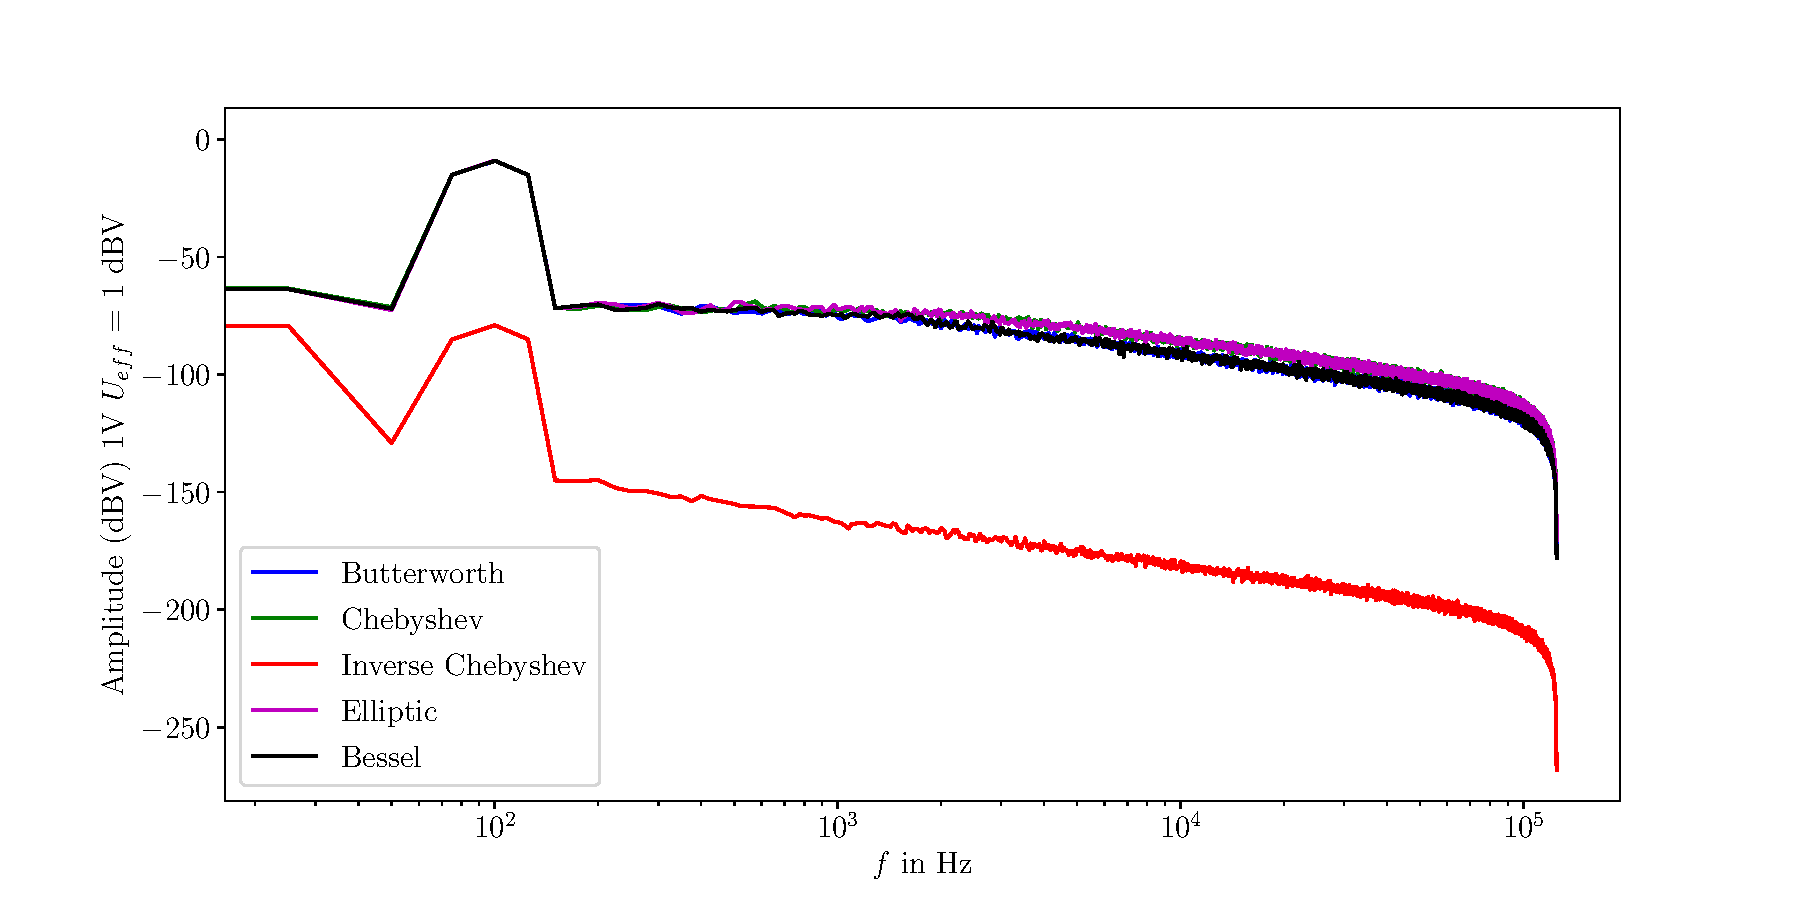
\includegraphics[width=\textwidth]{Paul/43aAll.pdf}
    \caption{Fourierspektrum verschiedene Tiefpassfilter}
    \label{fig:43aAll}
\end{figure}

In Abbildung \ref{fig:43aAll} fällt auf, dass sich Elliptic- und Chebyshevfilter fast deckungsgleich überlagern. Auch Butterworth- und Besselfilter sind auch fast deckungsgleich mit den oben genannten lediglich für Frequenzen zwischen ca. $10^3$ Hz und $10^5$ Hz divergieren sie geringfügig. Am stärksten weicht der inverse Chebyshevfilter von den anderen ab. Der Verlauf ist sehr ähnlich, nahezu parallel, jedoch ist sie Kurve nach unten verschoben. \\

\newpage
Außerdem soll  für jede Filterkurve der 3dB-Punkt und die Steigung, für große Frequenzen bestimmt werden.
Hierfür wurde für jede Filterkurve ein eigenes Diagramm erstellt, um das graphische Ablesen einfache zu gestalten.
Anhang?


\begin{figure}[h]
    \centering
    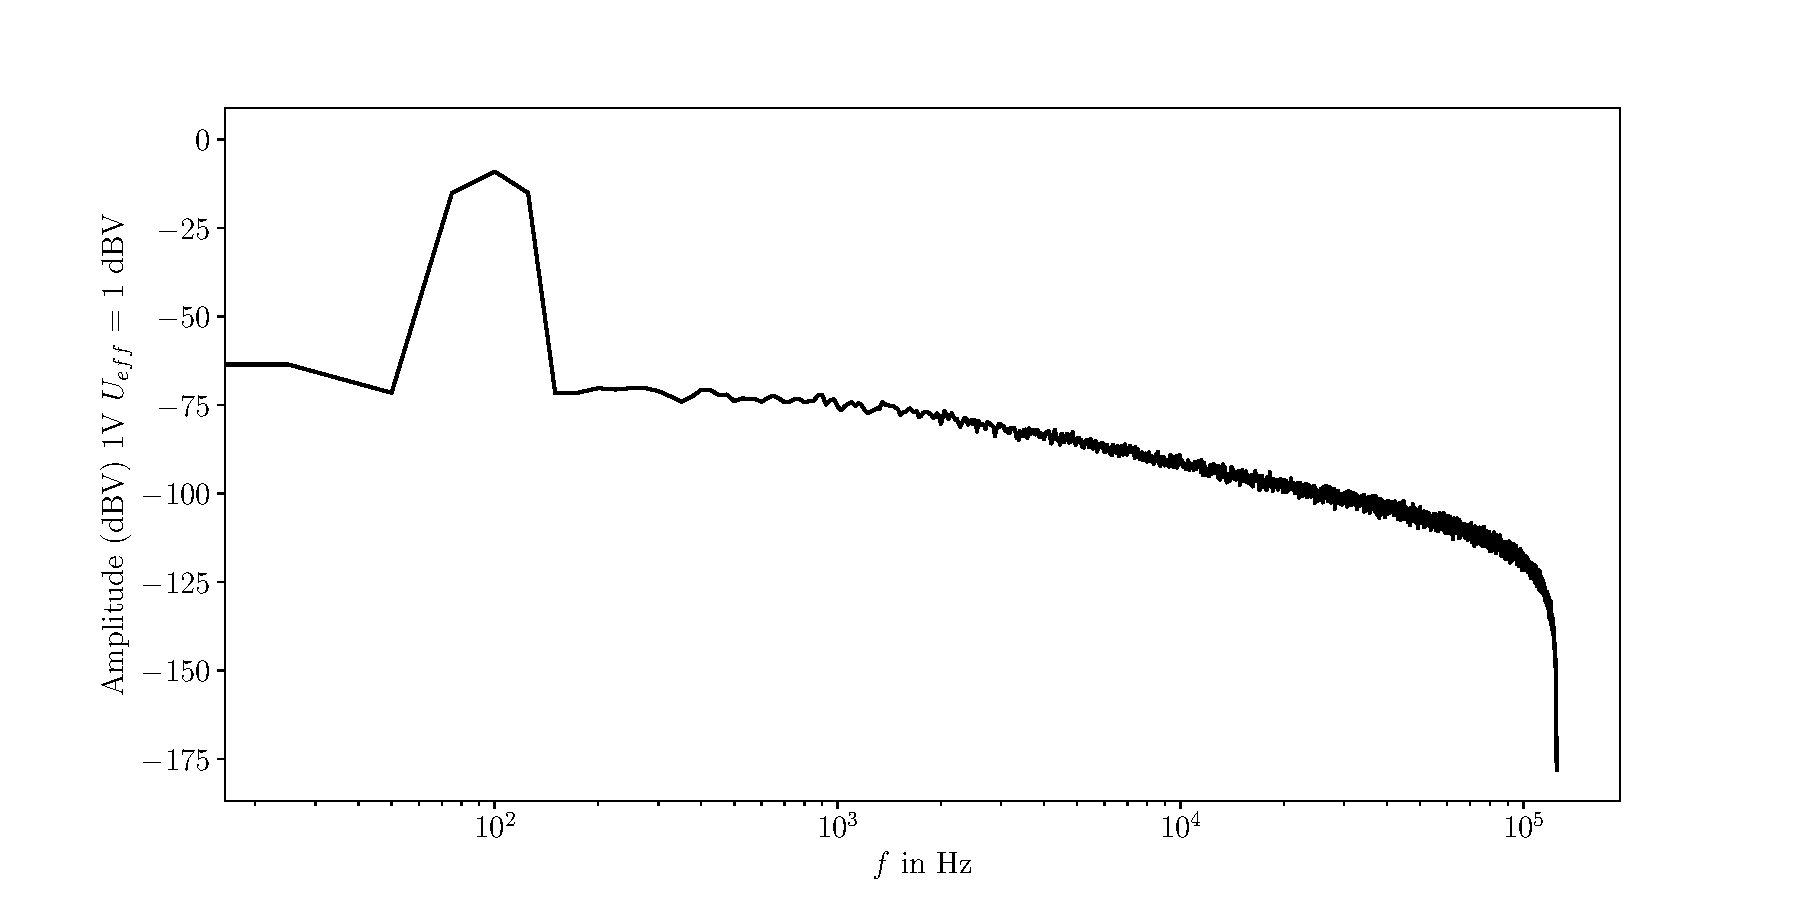
\includegraphics[width=\textwidth]{Paul/43aBu.pdf}
    \caption{Fourierspektrum des Butterworthfilter}
\end{figure}


\begin{figure}[h]
    \centering
    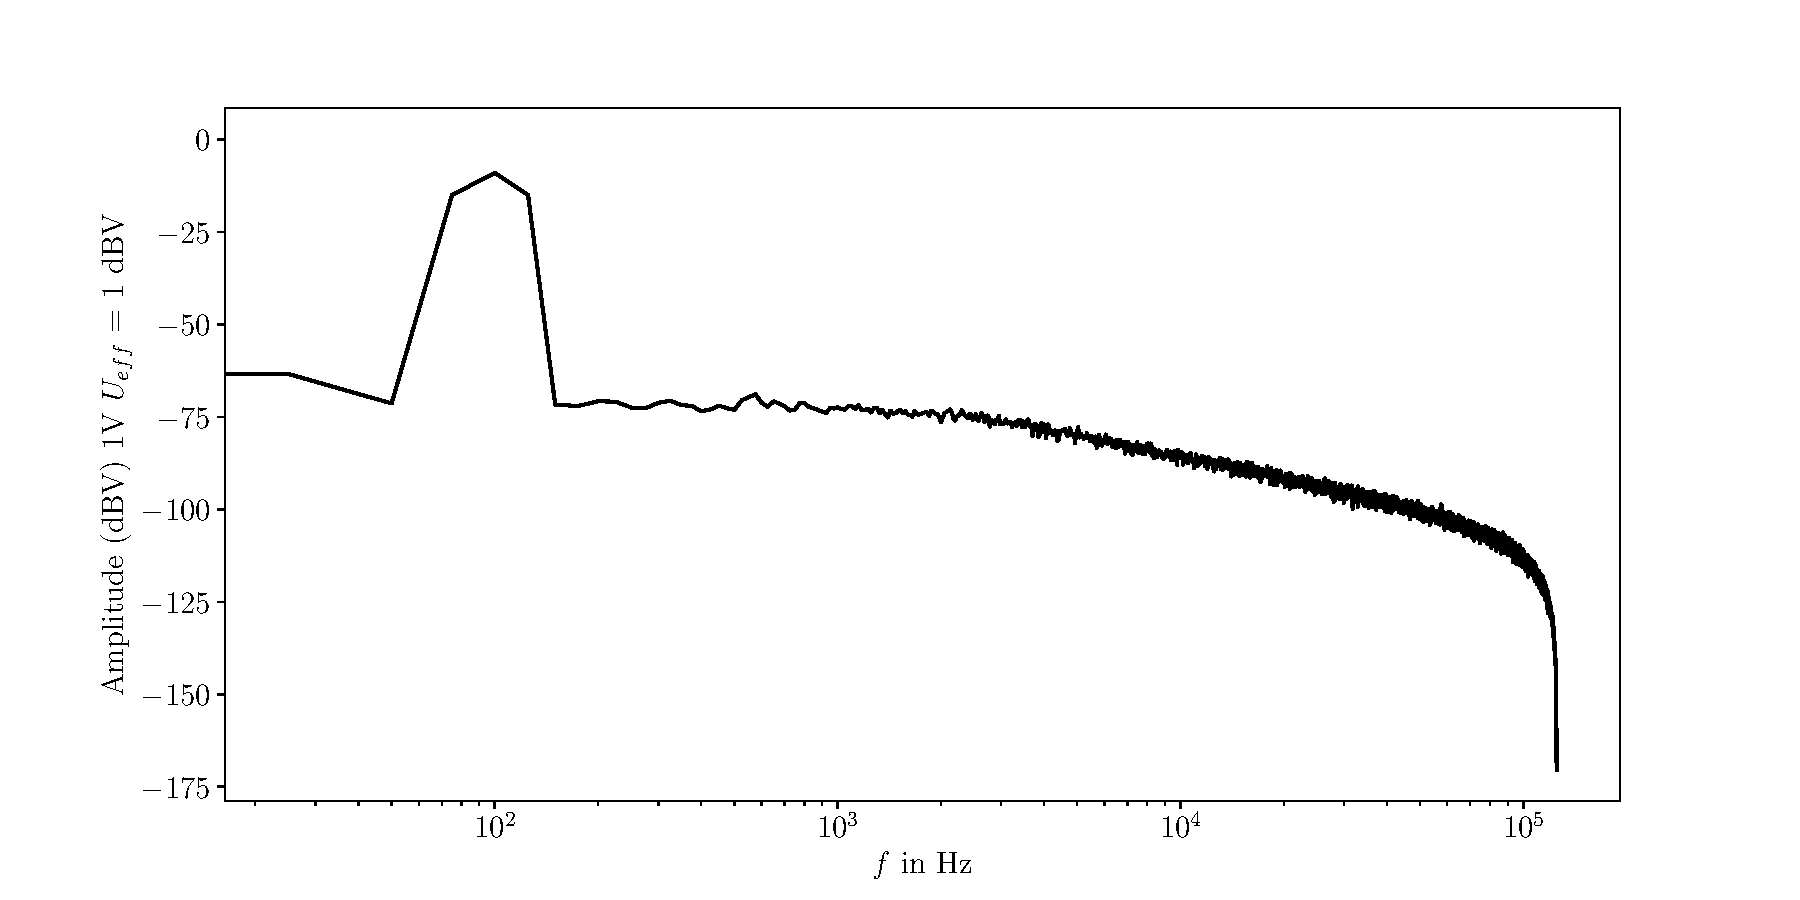
\includegraphics[width=\textwidth]{Paul/43aCh.pdf}
    \caption{Fourierspektrum des Chebyshevfilter}
\end{figure}

\newpage
\begin{figure}[h]
    \centering
    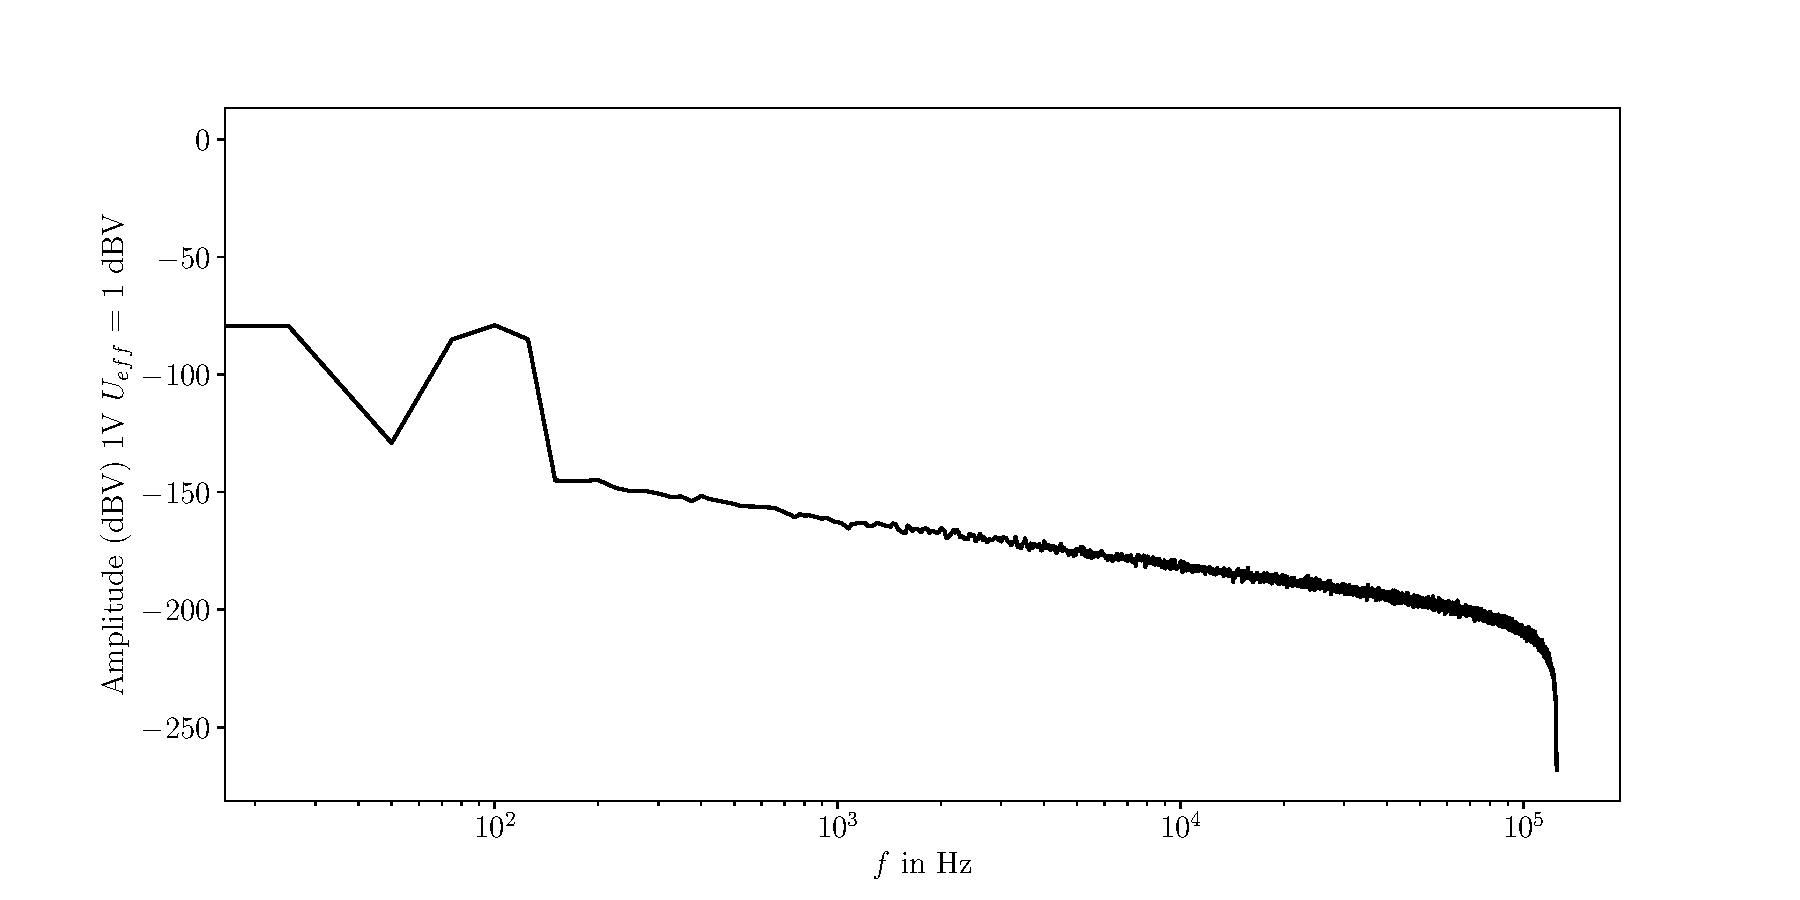
\includegraphics[width=\textwidth]{Paul/43aInCh.pdf}
    \caption{Fourierspektrum des inversen Chebyshevfilter}
\end{figure}


\begin{figure}[h]
    \centering
    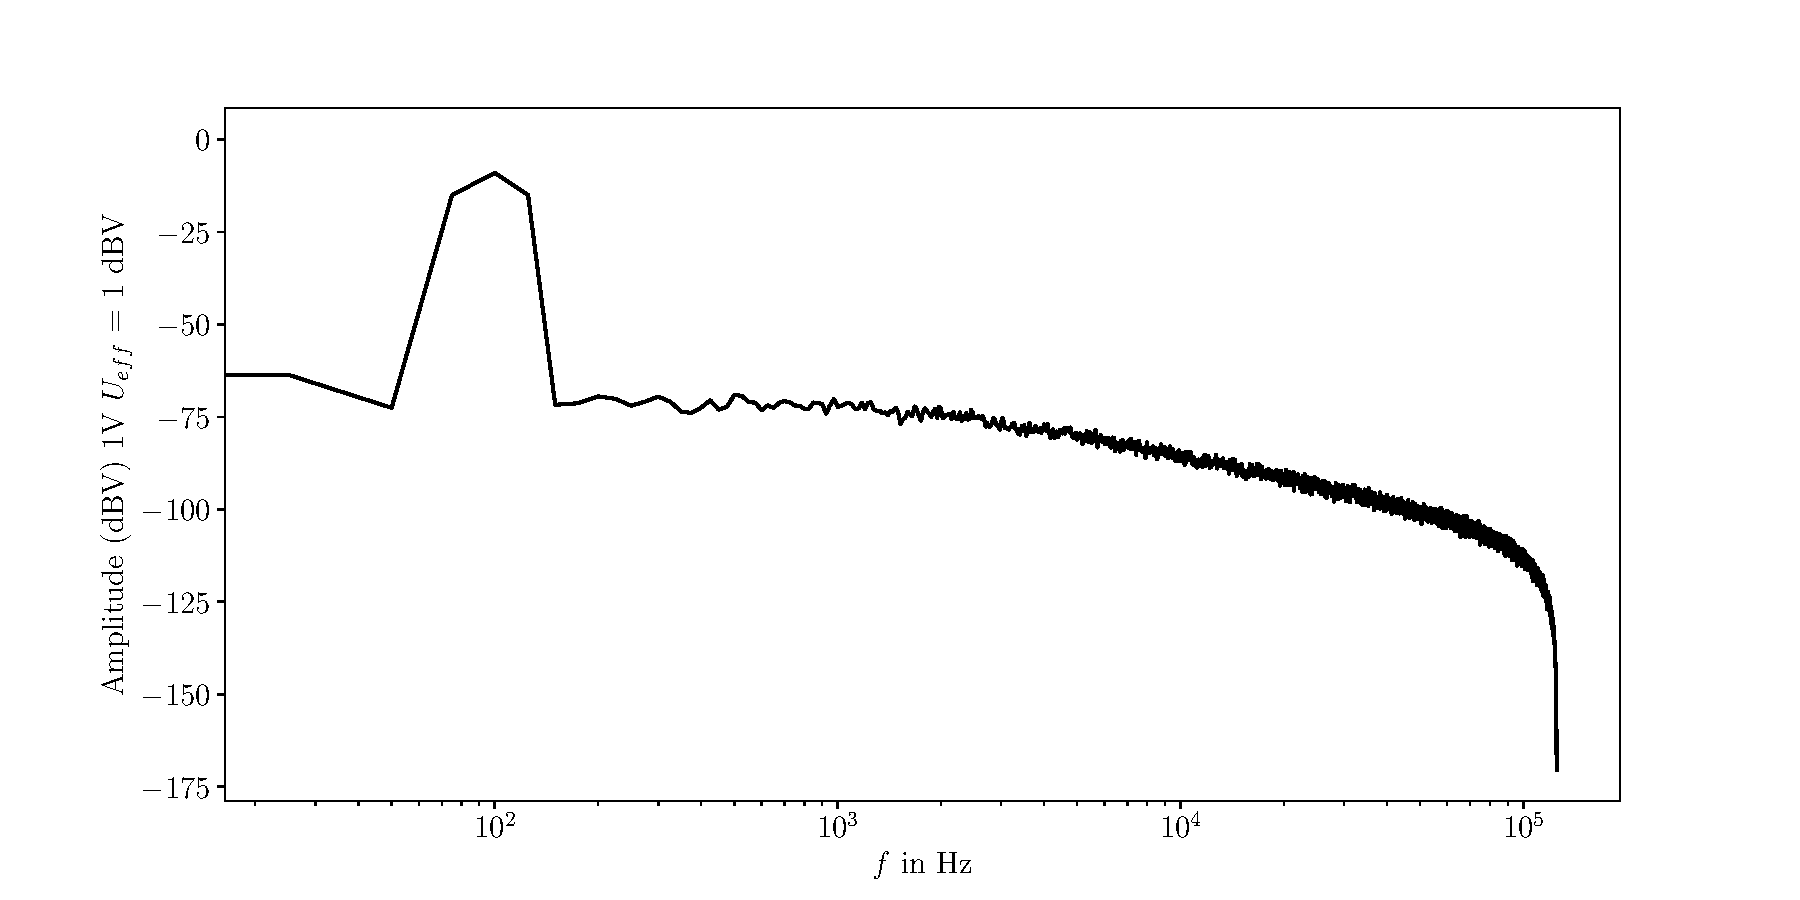
\includegraphics[width=\textwidth]{Paul/43aEl.pdf}
    \caption{Fourierspektrum des Ellipticfilter}
\end{figure}

\newpage
\begin{figure}[h]
    \centering
    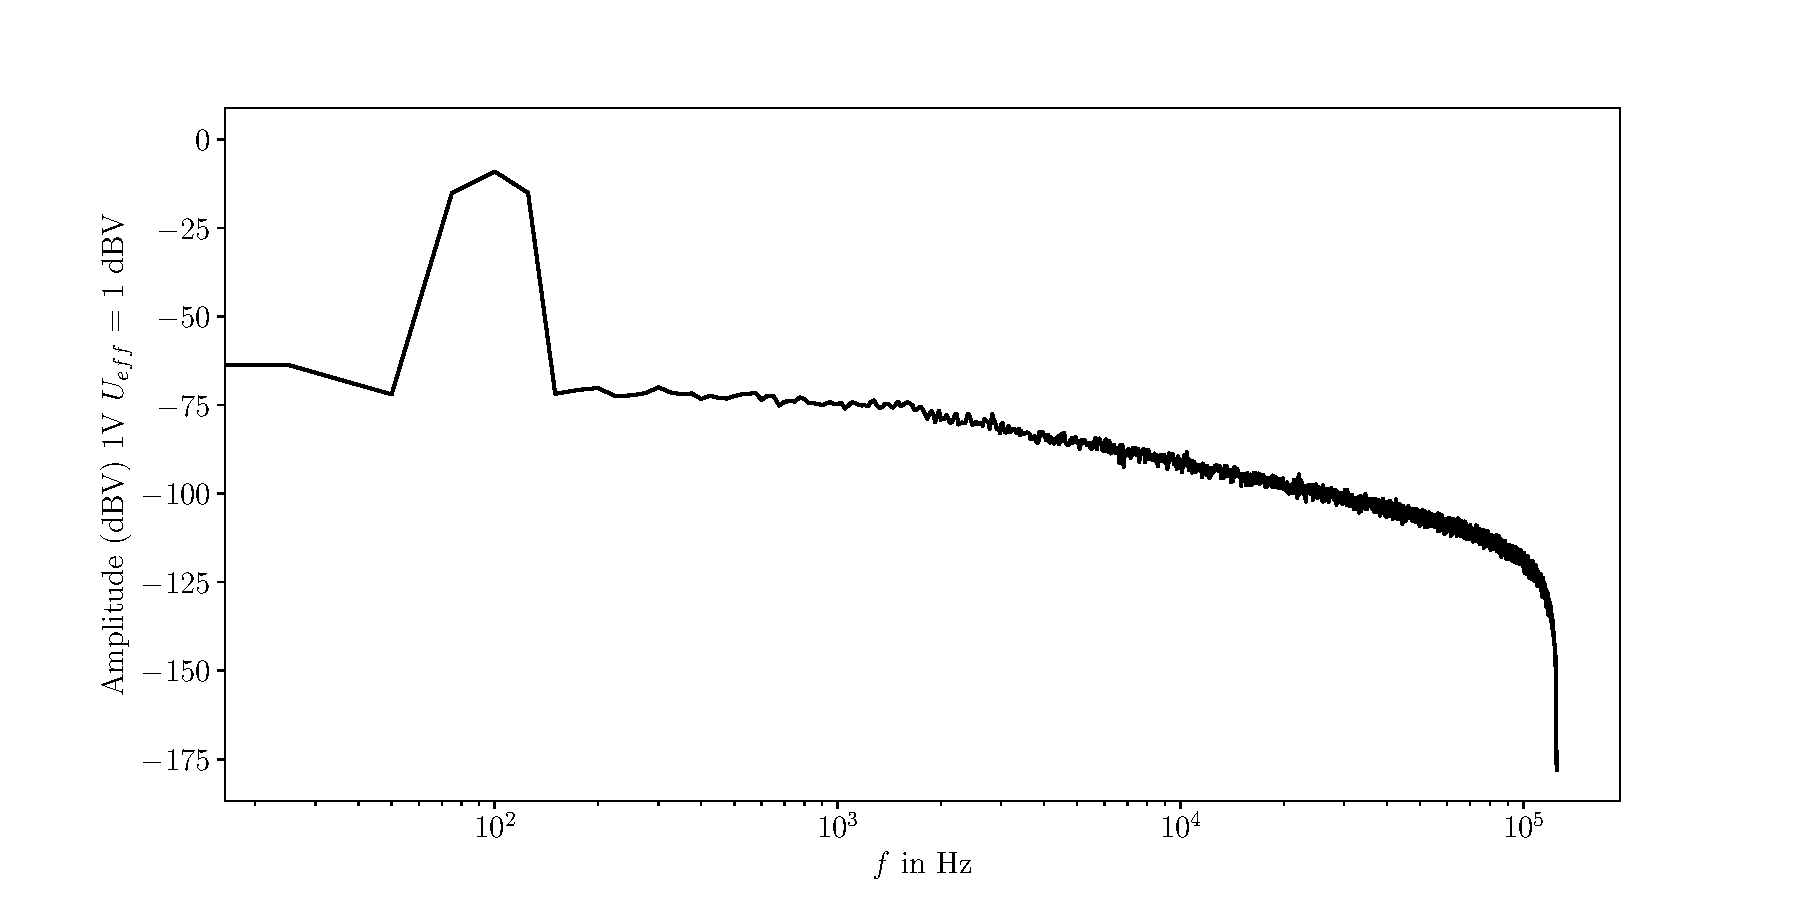
\includegraphics[width=\textwidth]{Paul/43aBe.pdf}
    \caption{Fourierspektrum des Bessselfilter}
\end{figure}

\newpage
\subsection{Filterwirkung auf Rechtecksignal}
In diesem Abschnitt soll die Wirkung verschiedener Filter auf ein Rechtecksignal ($f=100$ Hz) untersucht werden.

\begin{figure}[h]
    \centering
    \begin{subfigure}{\textwidth}
        \centering
        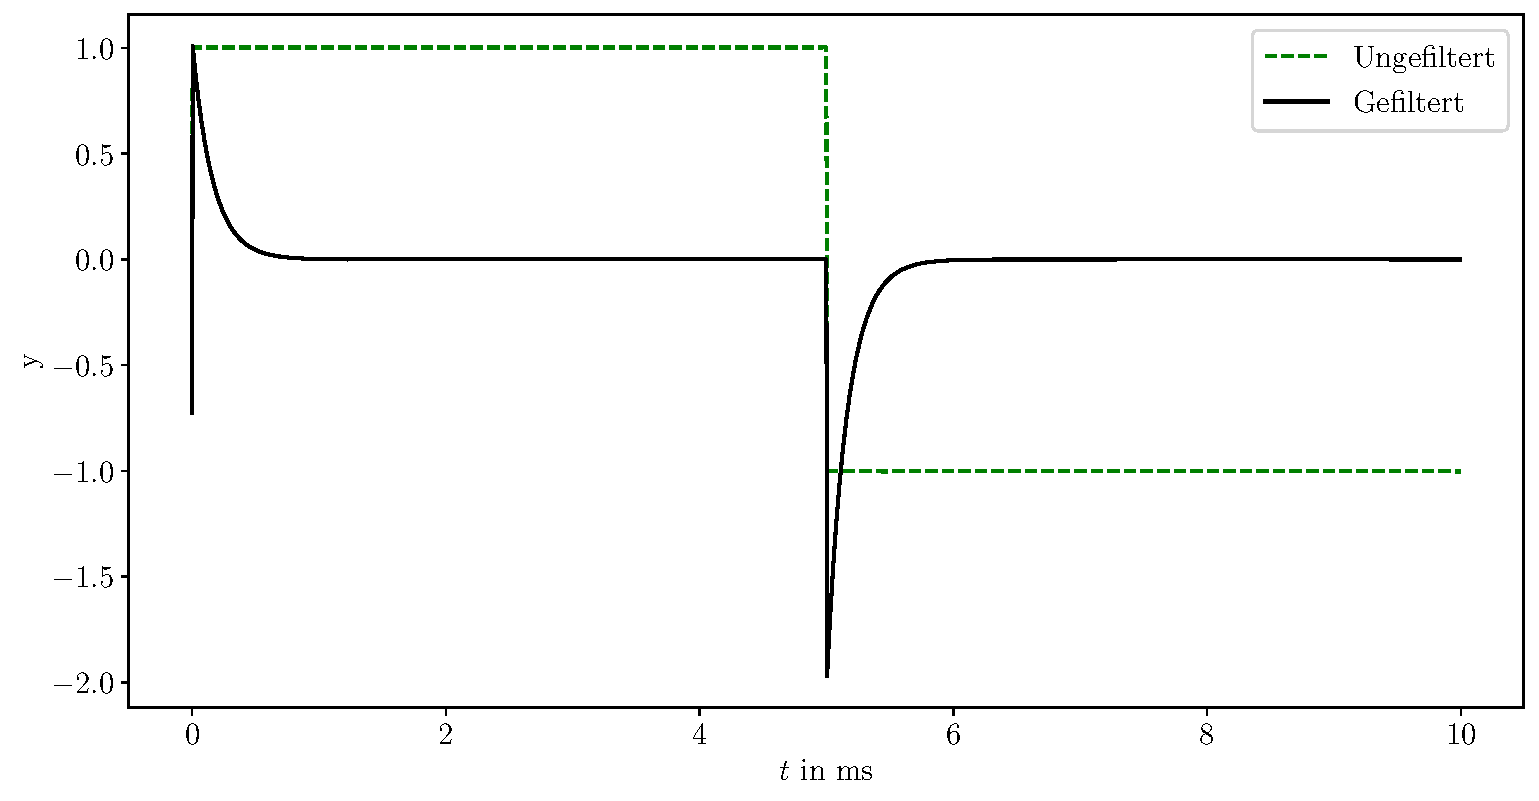
\includegraphics[width=\textwidth]{Paul/43bBuHi1S.pdf}
        \caption{Signal}
    \end{subfigure}\\
    \begin{subfigure}{\textwidth}
        \centering
        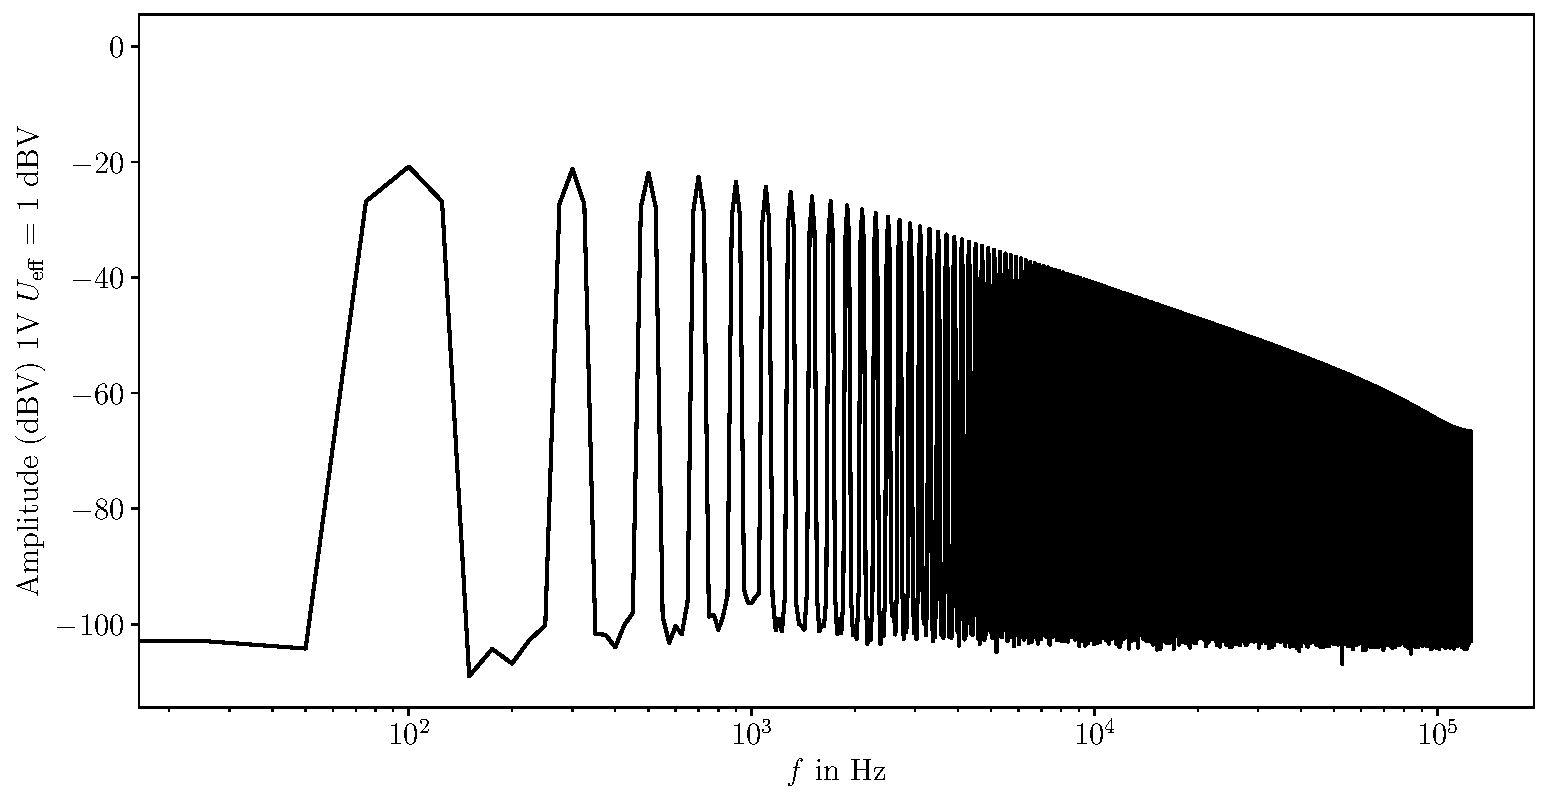
\includegraphics[width=\textwidth]{Paul/43bBuHi1F.pdf}
        \caption{Fourierspektrum}
    \end{subfigure}
    \caption{Butterworthfilter als Hochpass}
\end{figure}


\newpage
\begin{figure}[h]
    \centering
    \begin{subfigure}{\textwidth}
        \centering
        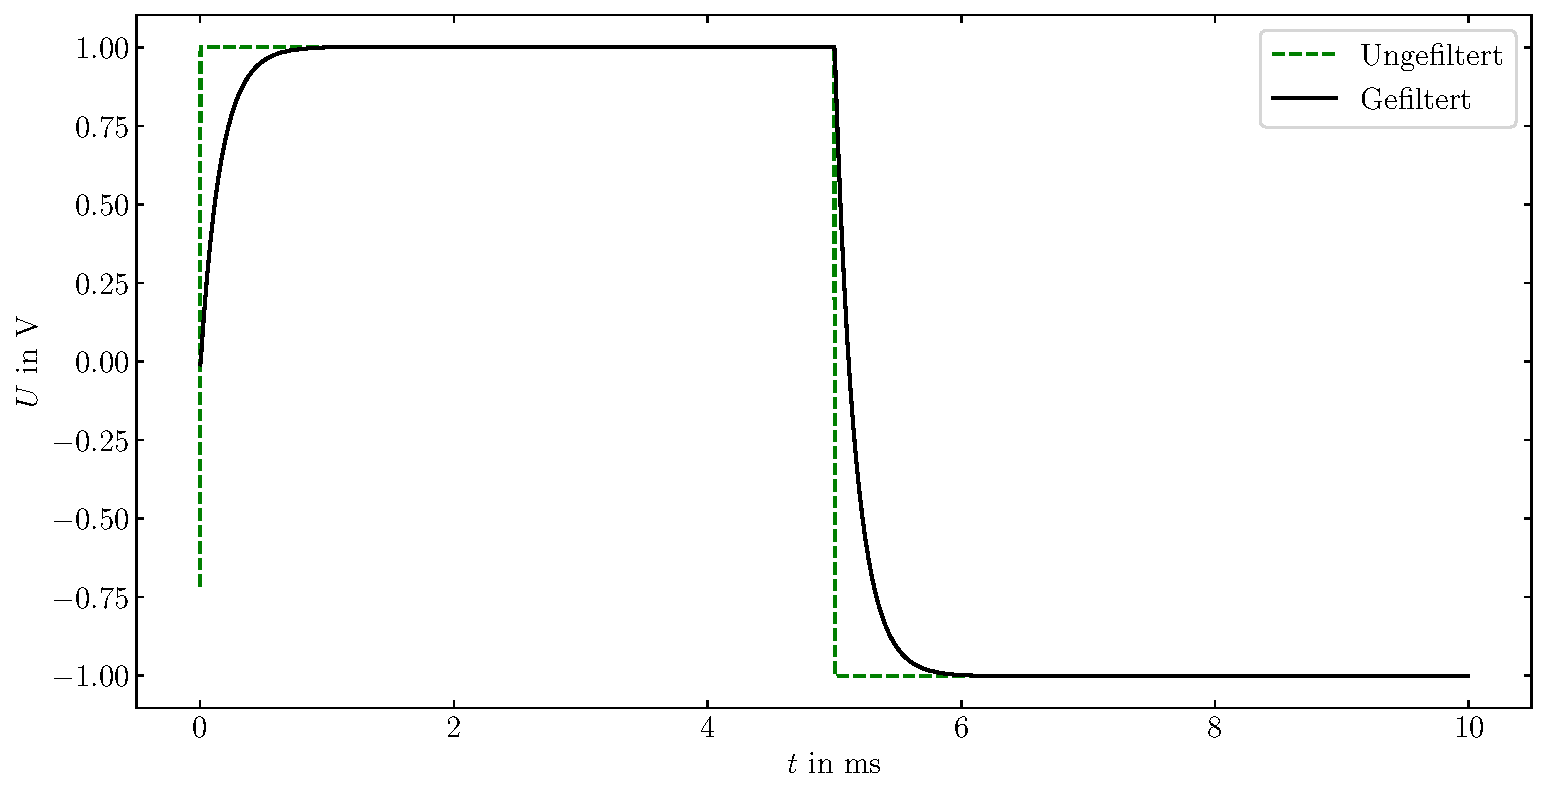
\includegraphics[width=\textwidth]{Paul/43bBuLo1S.pdf}
        \caption{Signal}
    \end{subfigure}\\
    \begin{subfigure}{\textwidth}
        \centering
        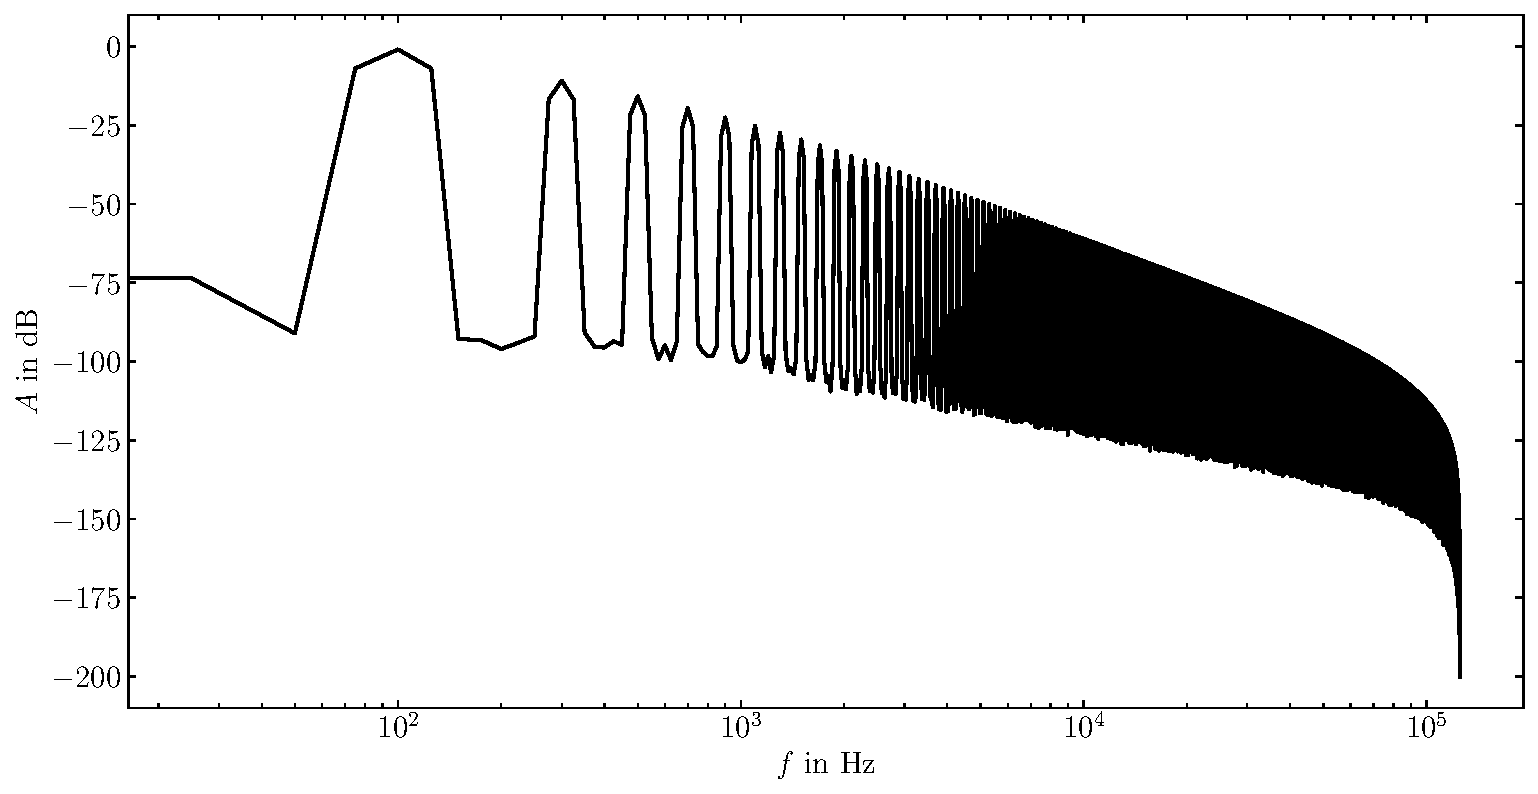
\includegraphics[width=\textwidth]{Paul/43bBuLo1F.pdf}
        \caption{Fourierspektrum}
    \end{subfigure}
    \caption{Butterworthfilter als Tiefpass}
\end{figure}


\newpage
\begin{figure}[h]
    \centering
    \begin{subfigure}{\textwidth}
        \centering
        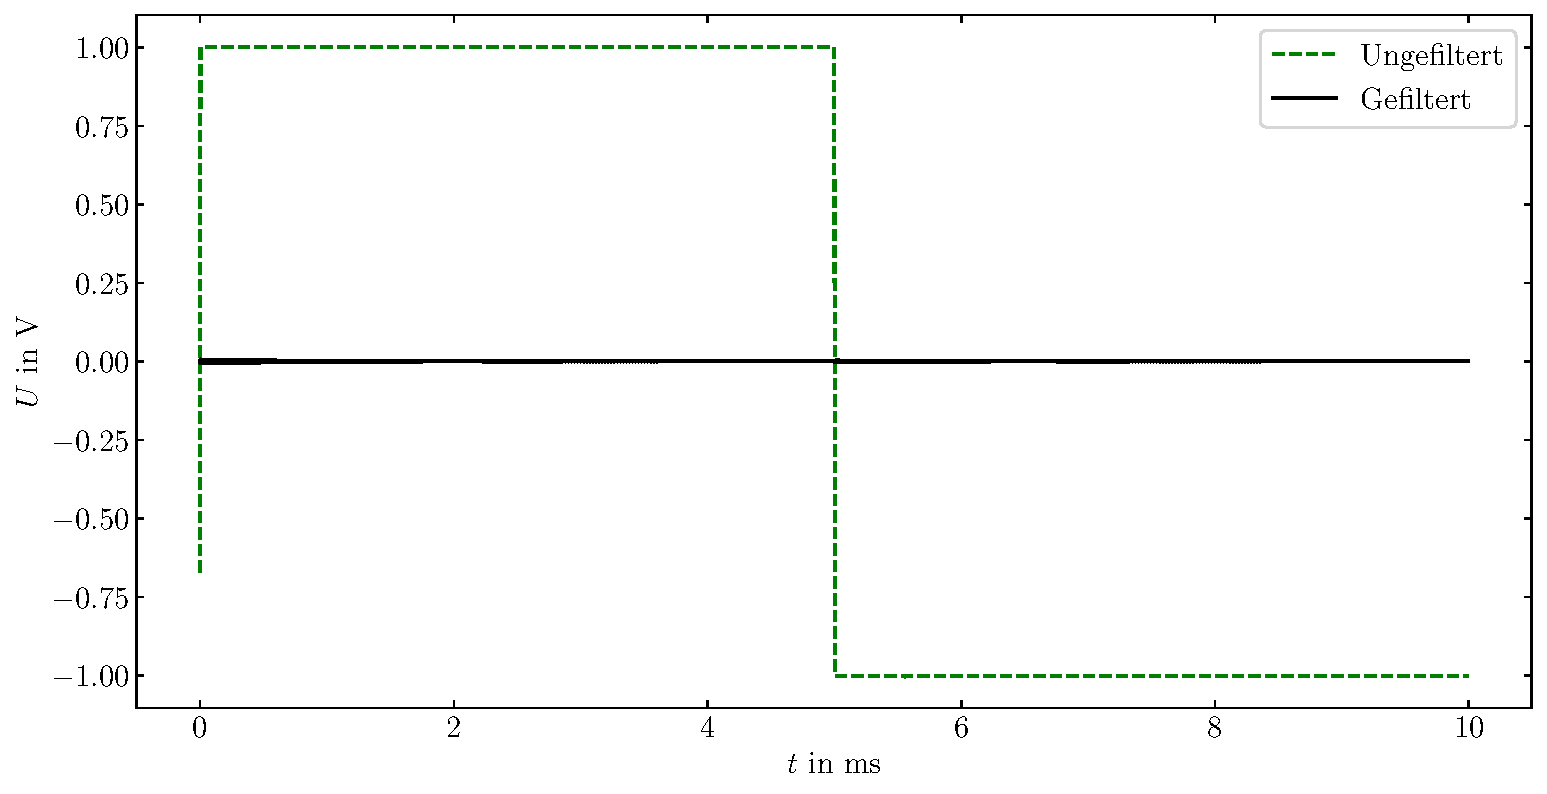
\includegraphics[width=\textwidth]{Paul/43bInChHi1S.pdf}
        \caption{Signal}
    \end{subfigure}\\
    \begin{subfigure}{\textwidth}
        \centering
        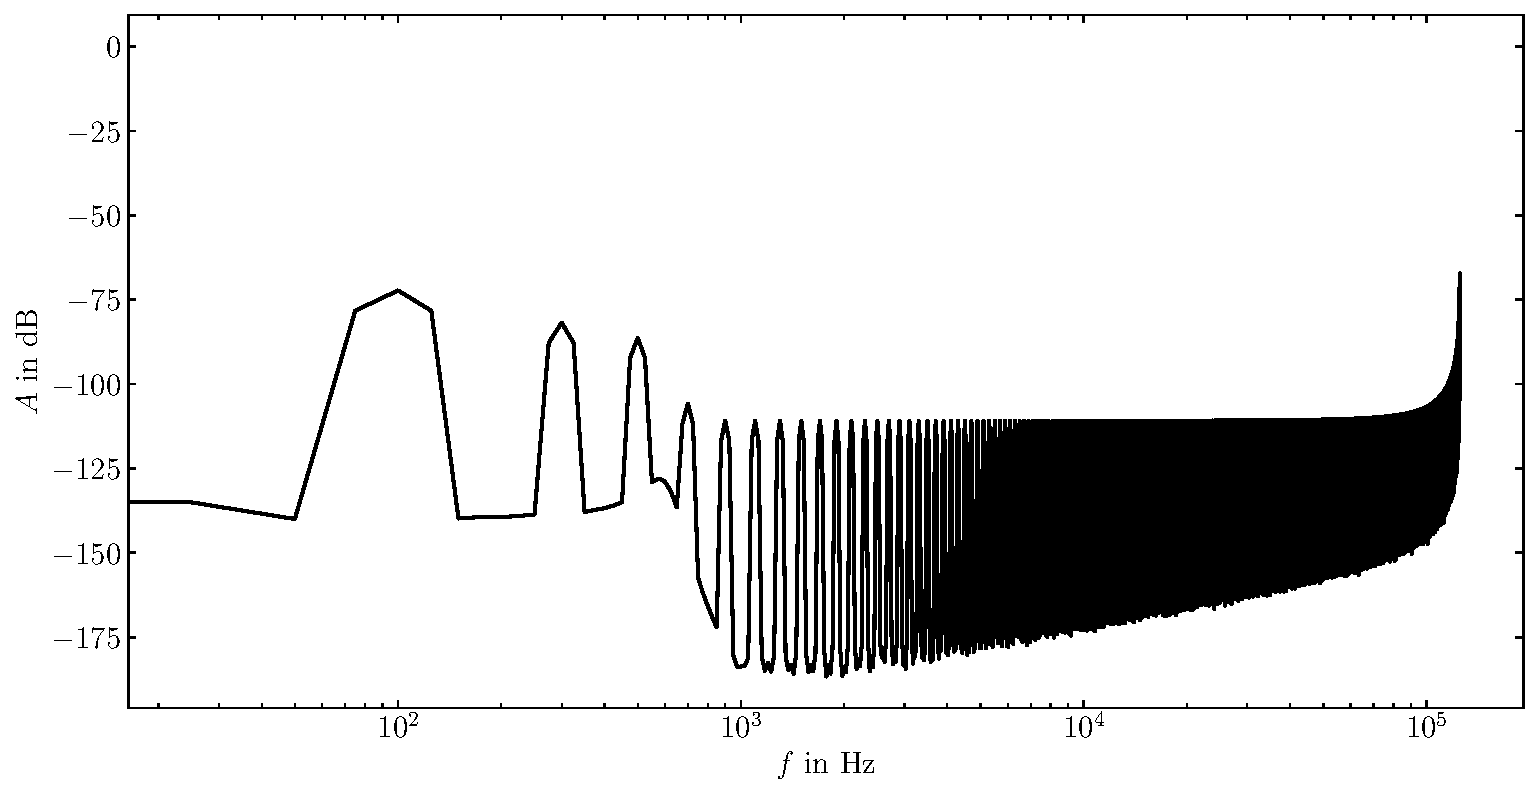
\includegraphics[width=\textwidth]{Paul/43bInChHi1F.pdf}
        \caption{Fourierspektrum}
    \end{subfigure}
    \caption{Inverser Chebyshevfilter als Hochpass}
\end{figure}


\newpage
\begin{figure}[h]
    \centering
    \begin{subfigure}{\textwidth}
        \centering
        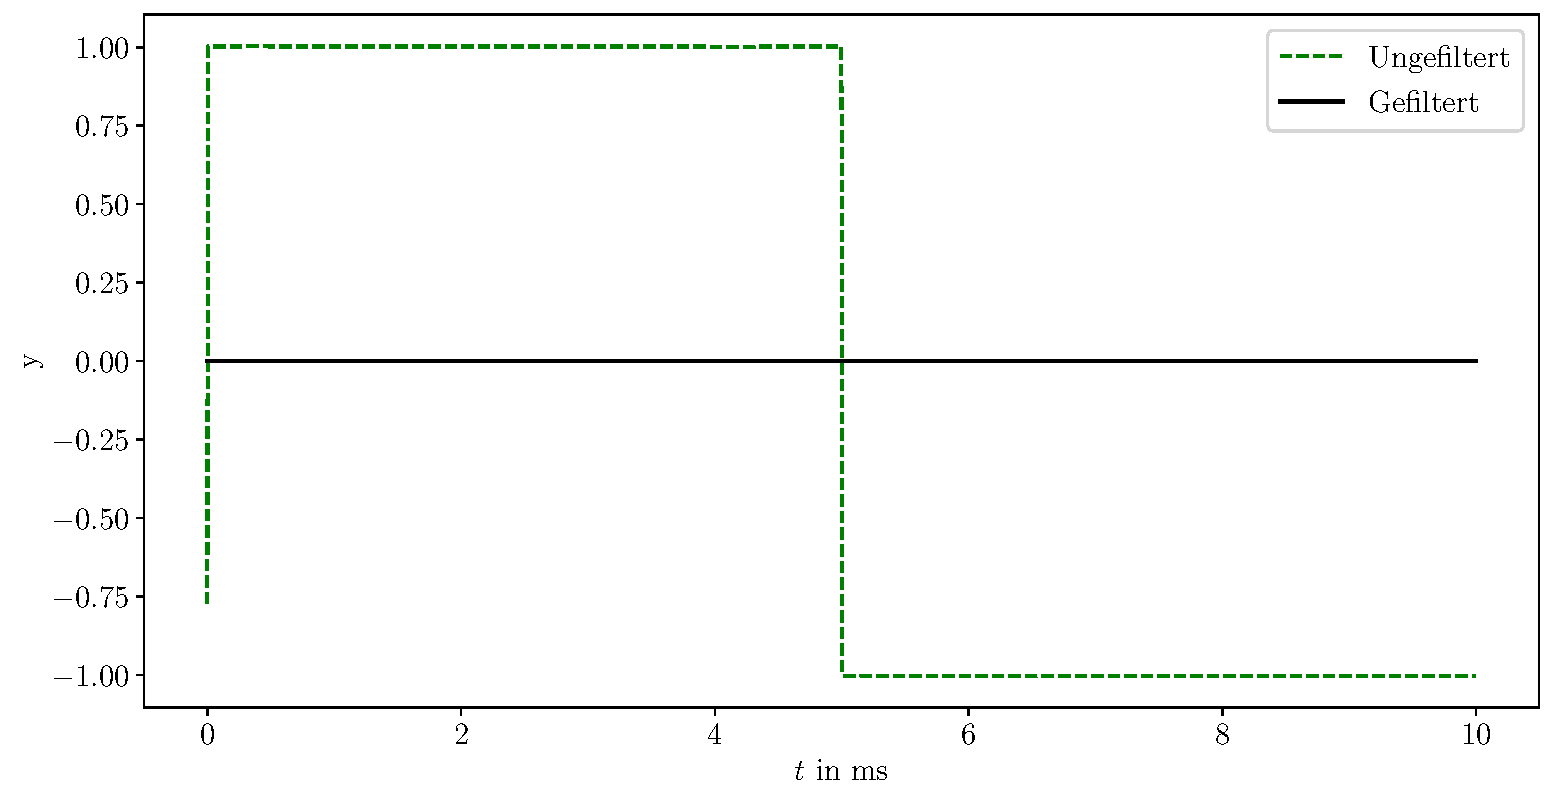
\includegraphics[width=\textwidth]{Paul/43bInChLo1S.pdf}
        \caption{Signal}
    \end{subfigure}\\
    \begin{subfigure}{\textwidth}
        \centering
        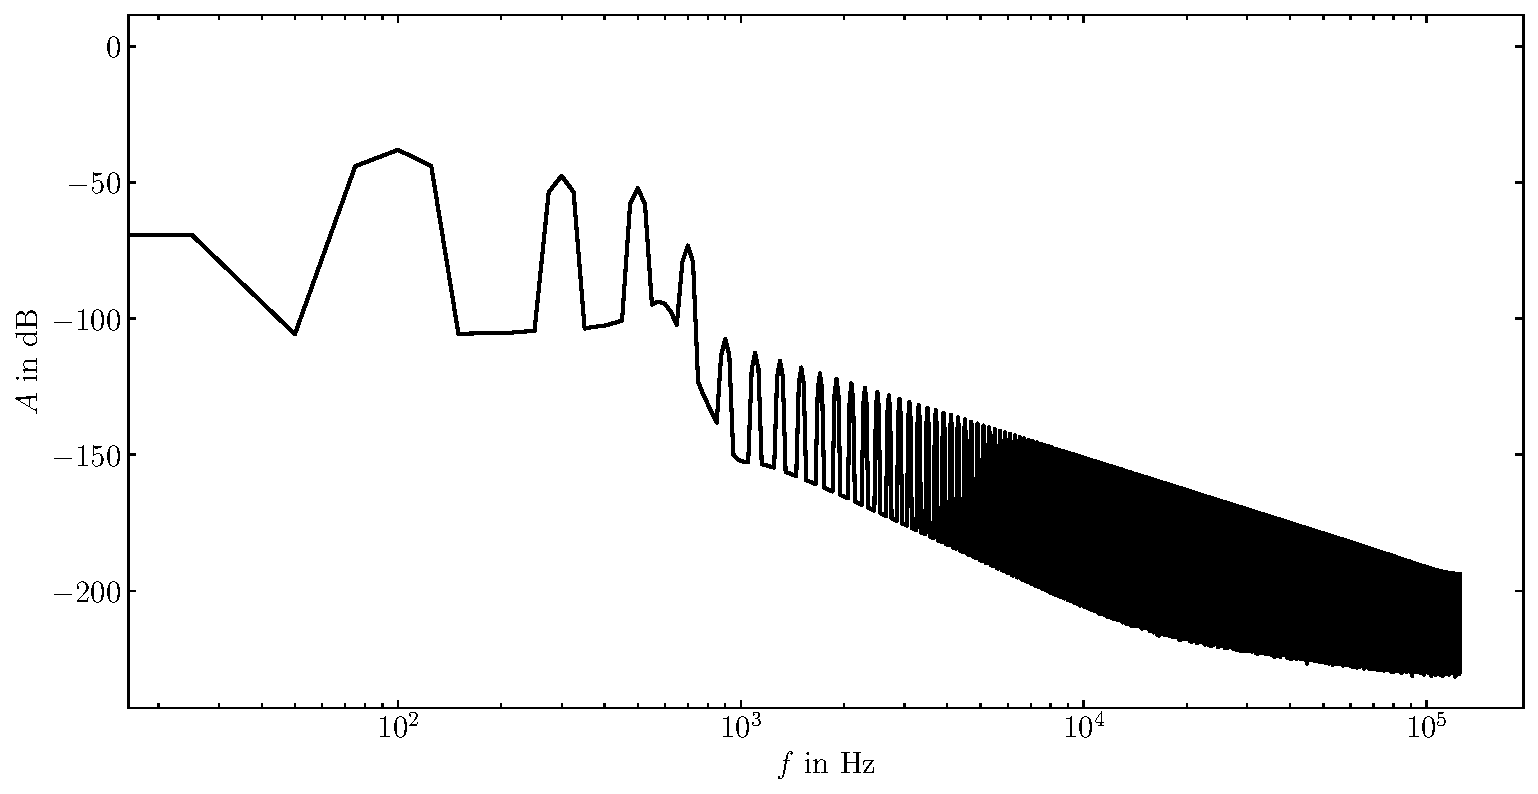
\includegraphics[width=\textwidth]{Paul/43bInChLo1F.pdf}
        \caption{Fourierspektrum}
    \end{subfigure}
    \caption{Inverser Chebyshevfilter als Tiefpass}
\end{figure}

\newpage
\subsection{Bandpass 4. Ordnung}


\subsection{Einfluss der Ordnung}


\subsection{Analoge vs. digitale Filterung}


\subsection{Vergleich Filterung und Mittelung}